% \section{Demonstration}

Der Nutzen des Konzeptes und dessen Umsetzung wird nachfolgend beispielhaft vorgestellt. Auf Basis der eingebauten Fehlerszenarien in der Demoanwendung soll der Mehrwert der erstellten Lösung evaluiert werden. Folgend wird näher beleuchtet, wie die drei Fehlerszenarien aufgedeckt werden können.

\subsection{Aufdecken des Szenarios \enquote{Keine Übersetzungen}}

Im Fehlerszenario \enquote{Keine Übersetzungen} werden in der Webanwendung die Übersetzungsschlüssel, statt der tatsächlichen Produktnamen, angezeigt (vgl. \autoref{subsec:keine-uebersetzungen}). Da es sich hierbei um einen Fallback handelt, wurde in der Webanwendung darauf verzichtet einen Fehler zu werfen. Dieser würde in Splunk hervorgehoben werden. Jedoch lassen sich in Splunk die Logdaten durchsuchen und so Sitzungen herausfinden, bei denen dieses Problem aufgetreten ist (vgl. \autoref{fig:keine-uebersetzungen_splunk-logs}). Darauf basierend konnten verwandte Logs derselben \enquote{Sitzung} inspiziert werden, allein anhand dessen konnte jedoch nicht das Fehlverhalten nachvollzogen werden. Aber die gefundene \texttt{shoppingCartId} bietet die Möglichkeit, damit in weiteren Systemen nachzuforschen.

\begin{figure}[H]
	\centering
	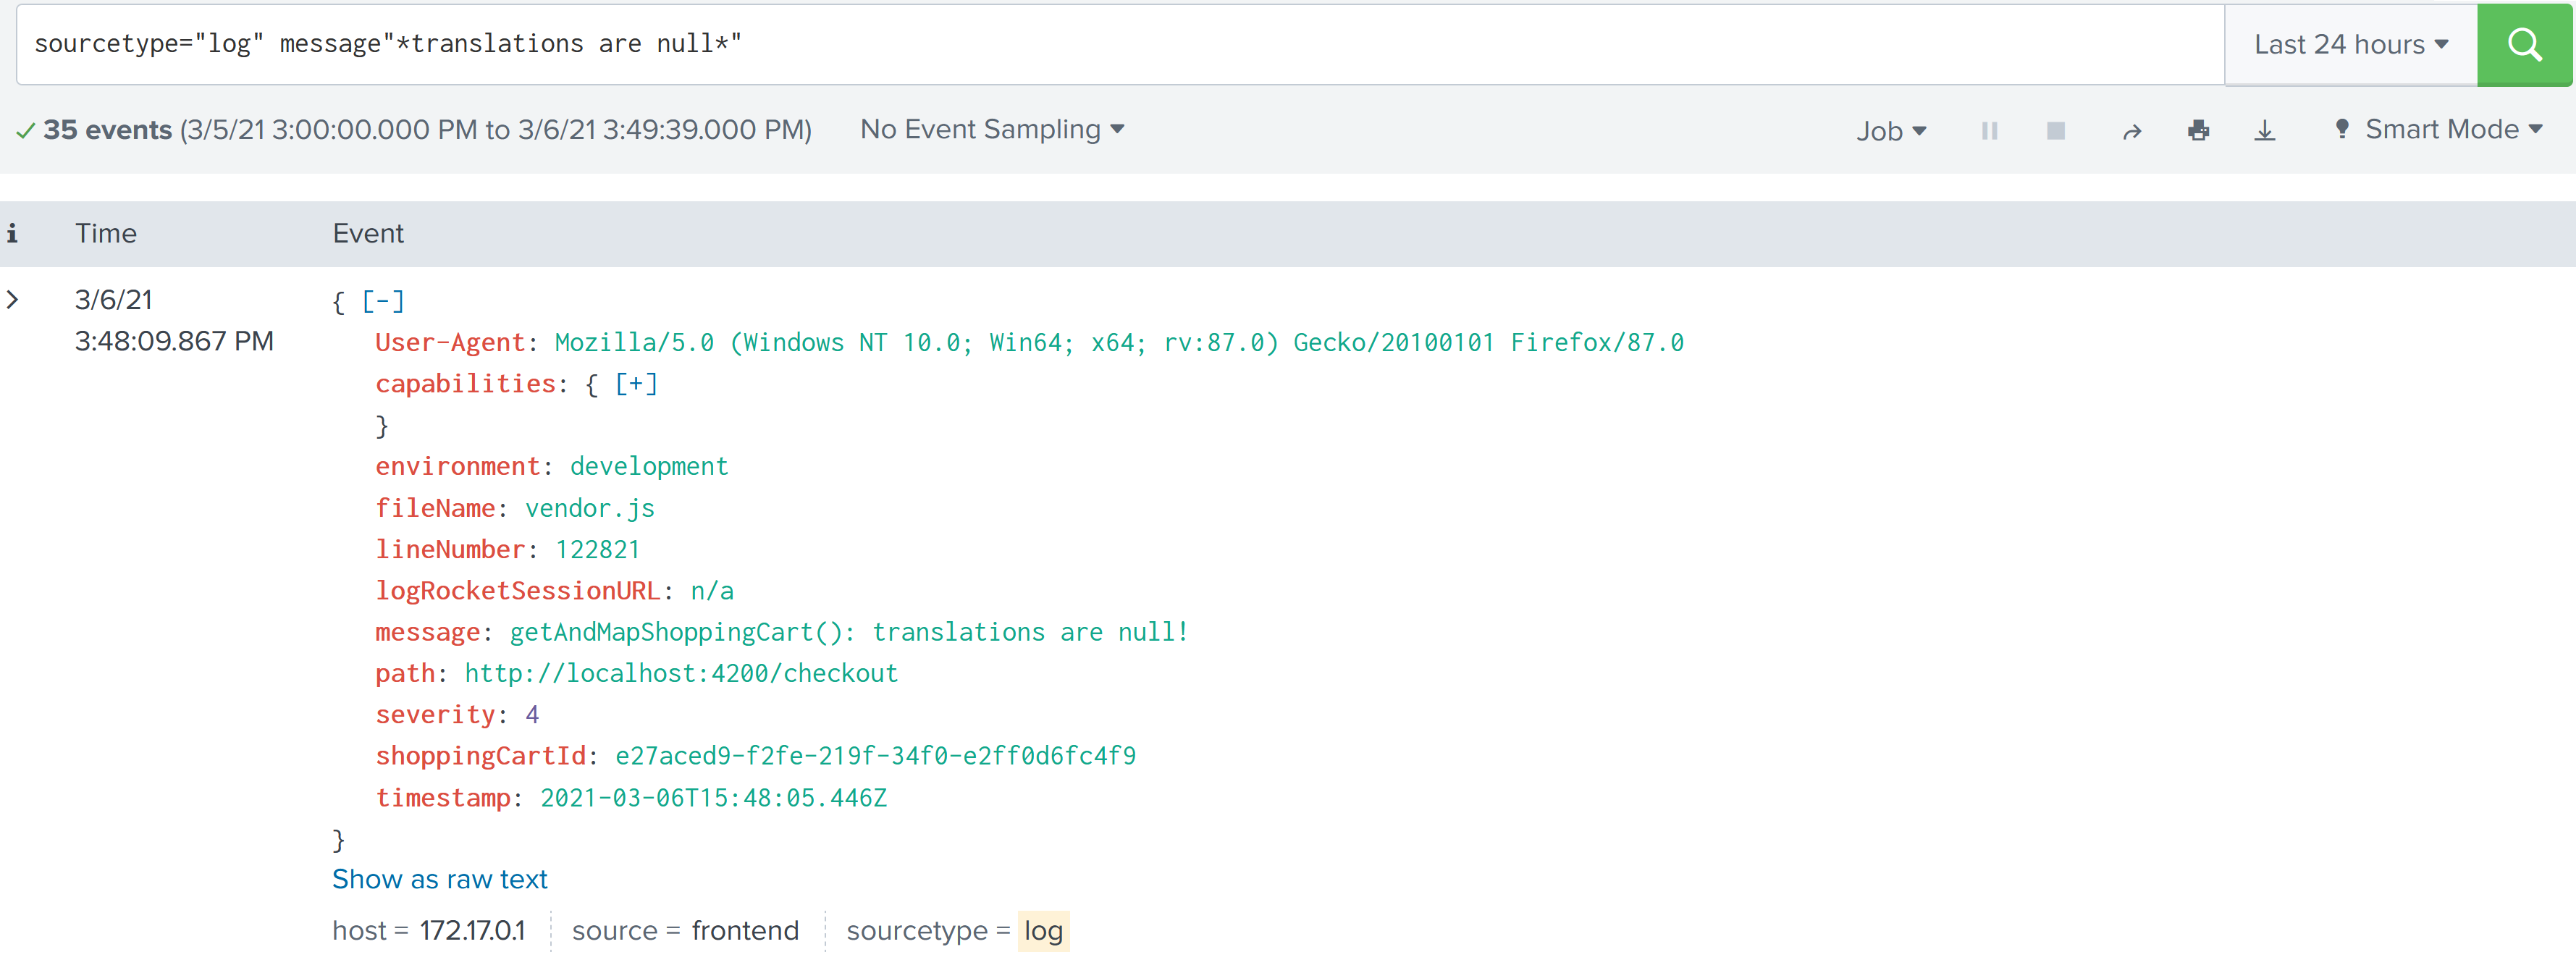
\includegraphics[width=1.00\linewidth]{img/05_ergebnis/keine-uebersetzungen_splunk-logs.png}
	\caption{Suche nach Logs zu fehlenden Übersetzungen in Splunk}
	\label{fig:keine-uebersetzungen_splunk-logs}
\end{figure}

\begin{wrapfigure}[14]{r}{0.50\textwidth}
\centering
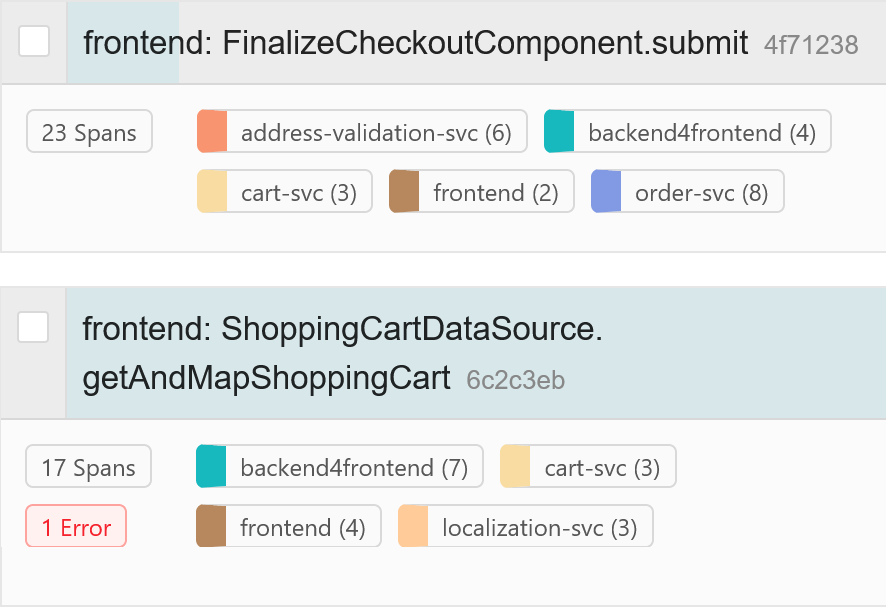
\includegraphics[width=\linewidth]{img/05_ergebnis/keine-uebersetzungen_jaeger_search-cropped.png}
\caption{Suchergebnisse in Jaeger zu spezieller \texttt{shoppingCartId}}
\label{fig:uebersetzungen_jaeger_search-cropped}
\end{wrapfigure}

In Jaeger lassen sich anhand der \texttt{shopping\-Cart\-Id} Traces finden (vgl. \autoref{fig:uebersetzungen_jaeger_search-cropped}). Einer dieser Traces ist mit einem Fehler markiert und wurde ursprünglich durch die Funktion \texttt{getAndMapShoppingCart} im Frontend ausgelöst. Dabei handelt es sich um eine Funktion, die die Warenkorb- sowie Übersetzungsdaten abruft und zusammengeführt.

Bei Klick auf den Trace wird das entsprechende Trace-Gantt-Diagramm geöffnet (vgl. \autoref{fig:keine-uebersetzungen_jaeger_detail}). Beim dargestellten Aufruf ist im Übersetzungsdienst ein Fehler aufgetreten, welcher vermutlich für die fehlenden Übersetzungen verantwortlich ist. Im Span ist zudem ein Log hinterlegt, welche einen Hinweis liefert: \texttt{configuration is invalid}. Weiterhin ist auch der genaue Kubernetes-Pod (\texttt{localization-svc-003}) zu sehen, der die Abfrage durchführte. Somit sind dem problemlösenden Entwickler viele notwendige Informationen geboten, die ihm dabei helfen das Problem zu lösen.

\begin{figure}[H]
	\centering
	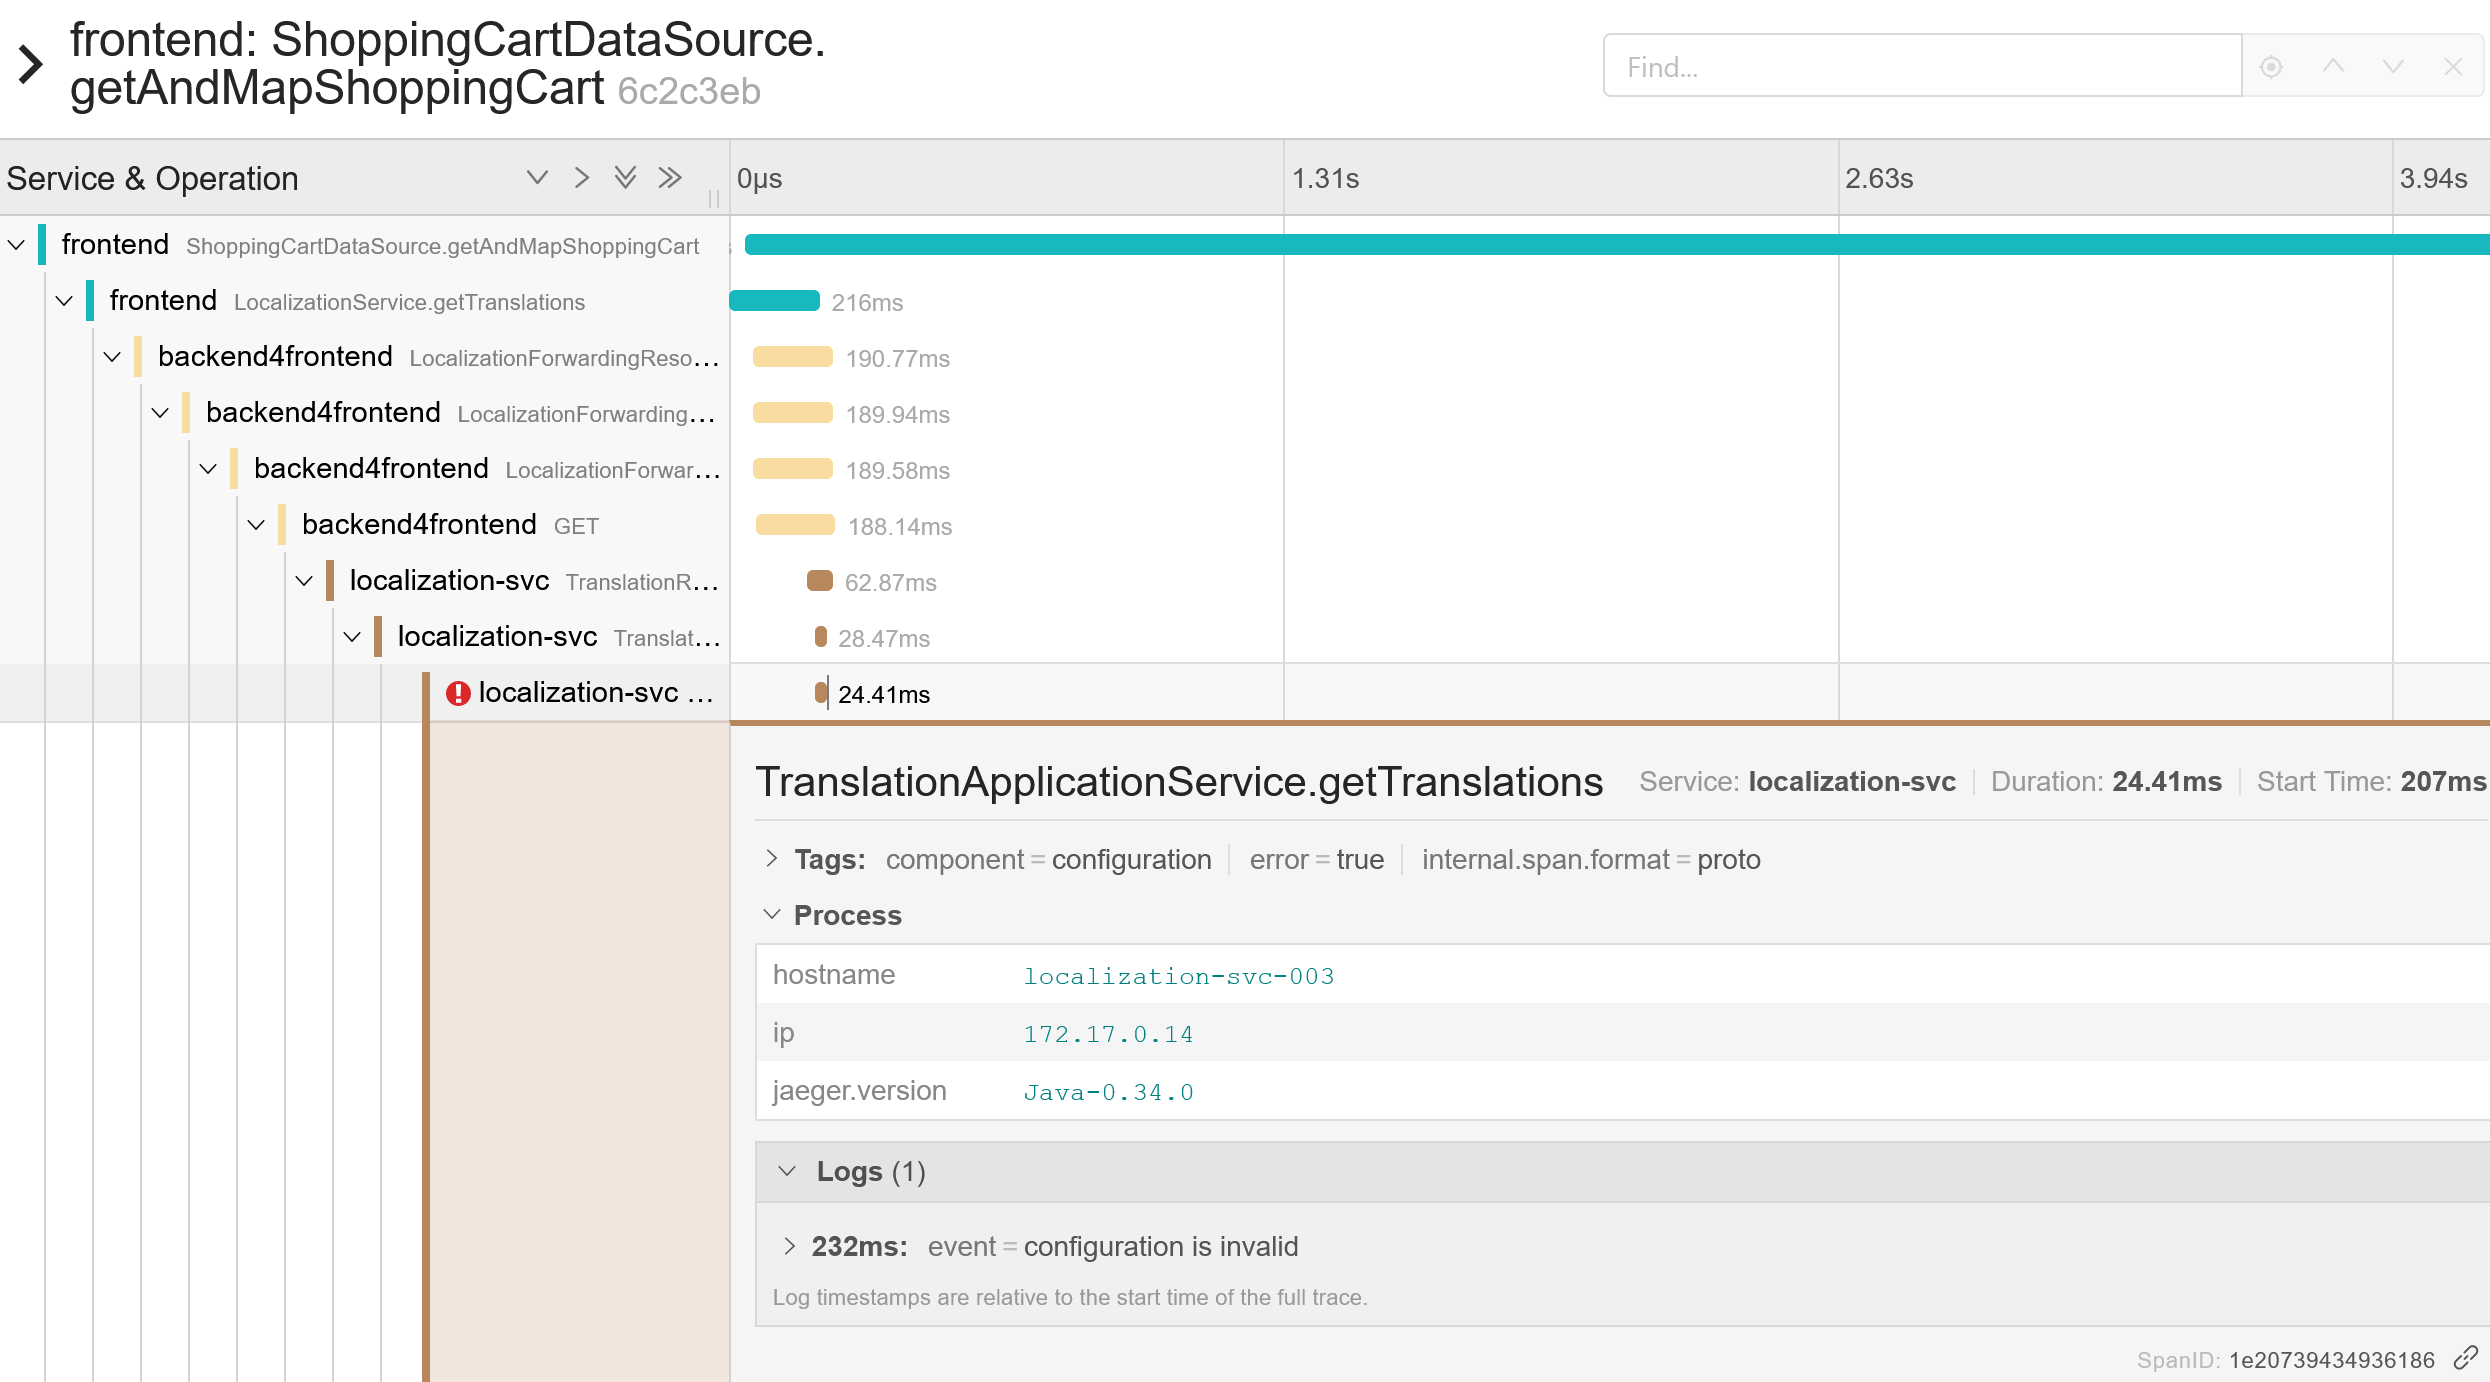
\includegraphics[width=1.00\linewidth]{img/05_ergebnis/keine-uebersetzungen_jaeger_detail.png}
	\caption{Ausschnitt des Traces zur Übersetzungsanfrage in Jaeger}
	\label{fig:keine-uebersetzungen_jaeger_detail}
\end{figure}

\subsection{Aufdecken des Szenarios \enquote{Ungültige Adressen sind gültig}}

Das Backend bietet angebundenen Systemen die Möglichkeit, eine Adresse zu validieren. Bei der Rechnungs- sowie der Lieferadresse sollte dies auch der Fall sein. Jedoch kommt es dazu, dass Nutzer ungültige Adressen angeben können und dies beim Absenden einer Bestellung zu einem Fehler führt (vgl. \autoref{subsec:ungueltige-adressen-sind-gueltig}). Durch die Suche in Splunk nach Logmeldungen der Angular-Komponente \texttt{Finalize\-Checkout\-Component} findet sich eine Fehlermeldung und eine entsprechende \texttt{shopping\-Cart\-Id}.

Mit Ausnahme der Fehlermeldung liefert Splunk keine sprechenden Informationen, sodass erneut auf Jaeger zurückgegriffen wird. In Jaeger findet sich ein entsprechender Trace (vgl. \autoref{fig:ungueltige-adressen-sind-gueltig_jaeger-detail}), der über die Situation Aufschluss gibt. Dabei ist zu erkennen, dass im Bestelldienst beide Adressen erneut validiert werden und die Anfrage bzgl. der Lieferadresse fehlschlägt. Auf Basis dieser Informationen kann der Entwickler erkennen, dass in der SPA keine Validierung für die Lieferadresse durchgeführt wird.

\begin{figure}[H]
	\centering
	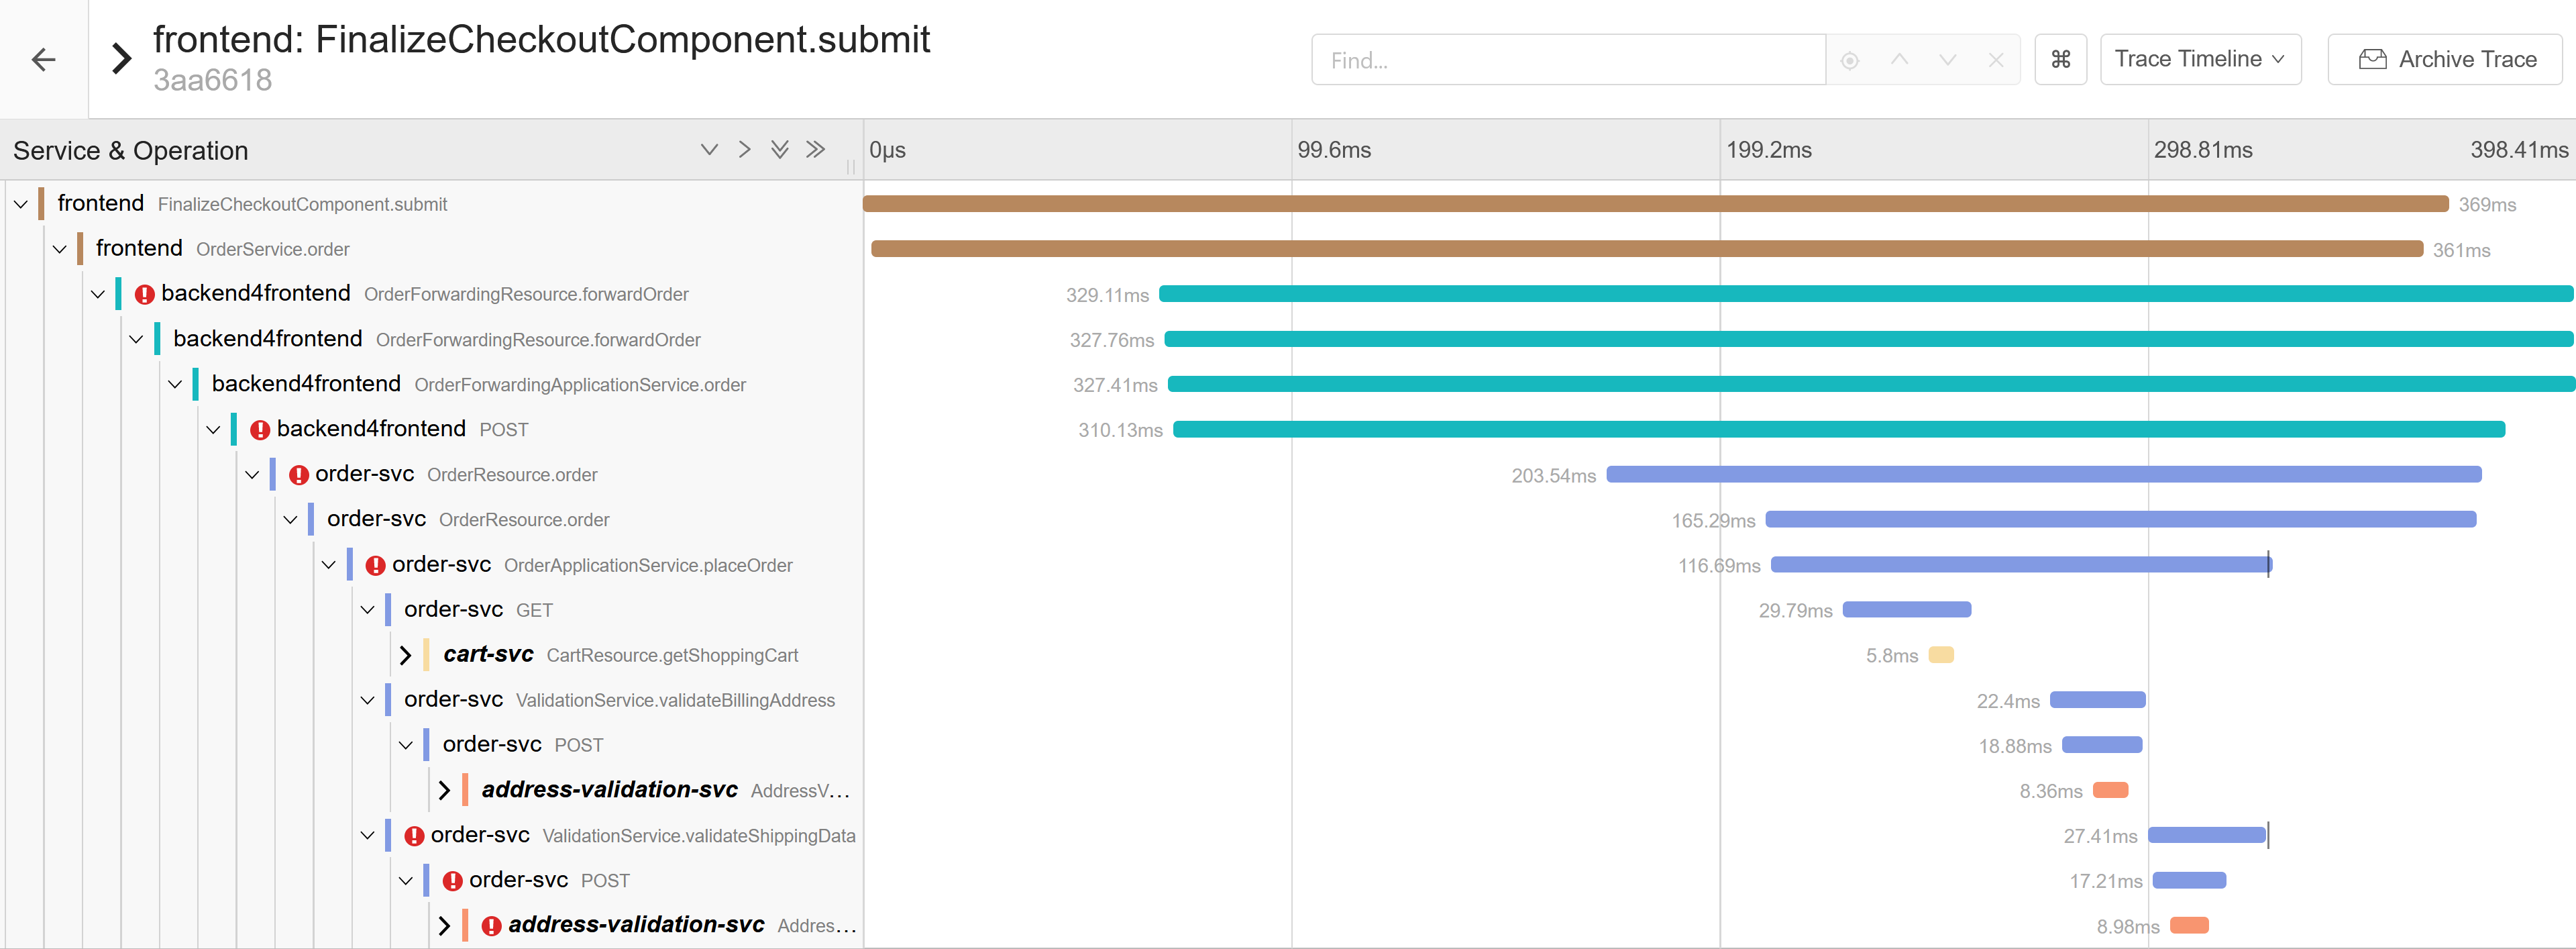
\includegraphics[width=1.00\linewidth]{img/05_ergebnis/ungueltige-adressen-sind-gueltig_jaeger-detail.png}
	\caption{Ausschnitt des Traces zur Bestellanfrage in Jaeger}
	\label{fig:ungueltige-adressen-sind-gueltig_jaeger-detail}
\end{figure}

\subsection{Aufdecken des Szenarios \enquote{Lange Verarbeitung}}

In diesem Szenario kommt es bei der Anzeige des Warenkorbes zu einer zeitlichen Verzögerung, sodass einige Sekunden vergehen, bis dieser sichtbar ist (vgl. \autoref{subsec:lange-verarbeitung}). In diesem Fall ist Splunk keine große Hilfe, da eine zeitliche Abfolge allein durch Logs schwer nachvollziehbar ist. Durch LogRocket ist das resultierende Verhalten gut nachzuvollziehen. Ein Video zu diesem Fehlerszenario ist im Anhang zu finden (siehe \autoref{sec:demo-logrocket}).

Auch in dieser Situation ist Jaeger ein wesentlicher Faktor. Anhand der Traces lassen sich nicht nur hierarchische Beziehungen nachvollziehen, sondern auch zeitliche. Eine Trace-Gantt-Visualisierung eines Traces, bei dem der Warenkorb abgerufen wird, ist in \autoref{fig:lange-verarbeitung_jaeger} zu betrachten. Dabei sticht hervor, dass der überwiegende Anteil der Zeit nicht in den Backendanfragen verloren geht, sondern durch die Operation \texttt{mapShoppingCart} im Frontend. Mithilfe dieser Informationen kann ein Entwickler nun hergehen und diese Operation verbessern.

\begin{figure}[H]
	\centering
	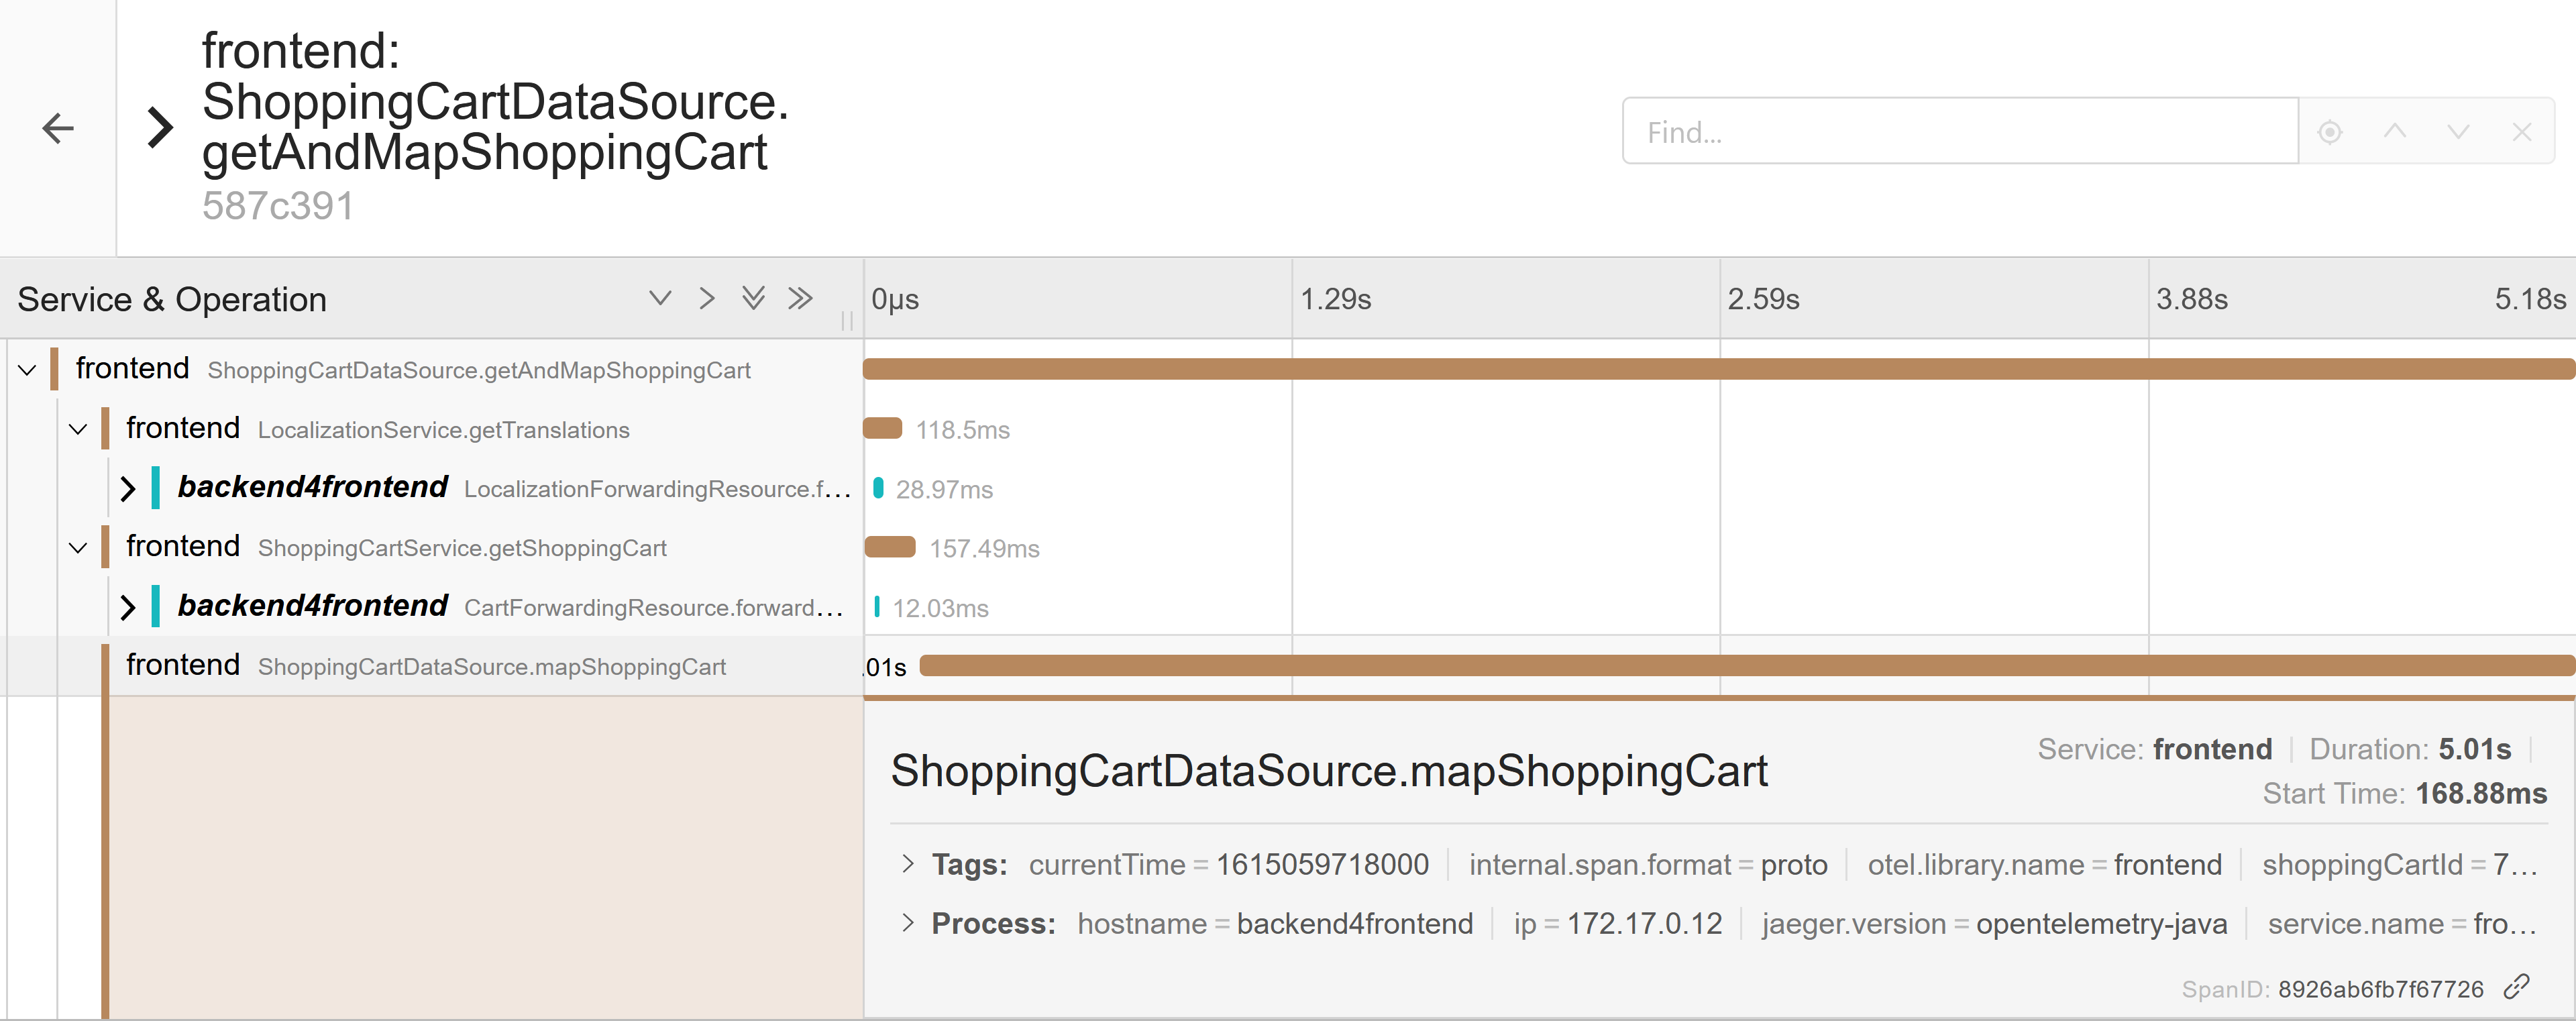
\includegraphics[width=1.00\linewidth]{img/05_ergebnis/lange-verarbeitung_jaeger.png}
	\caption{Ausschnitt des Traces zur Warenkorbanfrage in Jaeger}
	\label{fig:lange-verarbeitung_jaeger}
\end{figure}